%\magnification\magstephalf

\input sjnam
\input graphicx.sty

\def\f#1{{1\over #1^2}}
\def\ta#1{{x^{#1}\over #1!}}
\def\taa#1{\count255=#1 \advance\count255 by-1 
  {x^{\number\count255}\over #1!}}

\hsize 12.5cm
\nopagenumbers

\centerline{\hfont{HCR Dotum LVT Bold}{12pt} 바젤 문제}
\medskip
\centerline{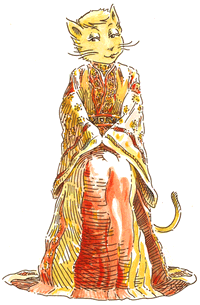
\includegraphics[width=3cm]{KTSmeta}}
$$1+\f2+\f3+\f4+\f5+\f6+\cdots$$
\bigskip\noindent 위 무한급수는 어떤 특정한 값으로 수렴한다는 것이 알려져 있고, 그 값은 놀랍게도 
$\pi^2\!/6$이다. 무한급수가 너무도 간단한 형식으로 표현되는 데에 놀랐고, 그 값에 $\pi$ 라는 
무리수가 들어간다는 데에 또 한 번 놀라게 된다. 정리하면, 다음과 같다.% 바젤 문제를 증명해보자.
$$1+\f2+\f3+\f4+\f5+\f6+\cdots={\pi^2\over6}.\eqno(1)$$
식(1)을 증명하는 바젤 문제는 수학의 정수론 분야에서 유명한 문제라고 한다.
이 문제는 볼로냐 대학의 교수였던 피에르토 멘골리가 1644년에 처음 제기
하여 볼로냐 문제로 불려야 맞겠으나, 이 문제를 세계에 널리 알려 
관심을 불러 일으킨 자코브 베르누이와 이 문제를 해결한 
오일러를 기리기 위해서 그들의 고향인 스위스의 도시, 바젤을 본따서 
바젤 문제로 불린다.

오일러는 이 문제를 어떻게 해결했을까? 오일러의 해결 방법이 유명한 이유는 오일러는
어려운 수학을 사용하지도 않고, 매우 기발한 아이디어로 바젤 문제를 해결했기 때문이다.
오일러는 쌩뚱맞게도 $\sin x=0$의 근을 구하는 데서 출발했다. 
$\sin x$의 근들은 잘 아다시피 $x=0$, $\pm\pi$, $\pm2\pi$, $\pm3\pi$, $\ldots$ 이다.
그렇다면 $\sin x/x=0$의 근은 무엇일까? 이는 $\sin x$의 근들과 일치하는데, 다만 분자는
$0$이 될 수 없으므로, 근들은 $x=\pm\pi$, $\pm2\pi$, $\pm3\pi$, $\ldots$이 된다.

이제 고등학교 혹은 대학교 수학시간에 테일러 급수라는 것을 기억에 떠올려보자.
우리의 기억이 맞다면, $\sin x$의 테일러 급수는 다음과 같다.
$$\sin x=x-\ta3+\ta5-\ta7+\cdots.\eqno(2)$$
위 식(2)의 양변을 $x$로 나누면, 다음의 식(3)를 얻는다.
$${\sin x\over x}=1-\taa3+\taa5-\taa7+\cdots.\eqno(3)$$
식(3)의 근들은 어떤 값들일까? 앞서 살펴보았듯이, 그 근들은 
$x=\pm\pi$, $\pm2\pi$, $\pm3\pi$, $\ldots$이다.
그런데, 어떤 방정식의 근이  
$a$, $b$, $c$라면, 그 방정식은 다음과 같이 쓸 수 있다.
$$(x-a)(x-b)(x-c)=0.\eqno(4)$$
따라서, 식(3)은 다음과 같이 나타낼 수 있다.
$$\displaylines{\qquad1-\taa3+\taa5-\taa7+\cdots=\hfill\cr
\noalign{\smallskip}
\hfill(x-\pi)(x+\pi)(x-2\pi)(x+2\pi)(x-3\pi)(x+3\pi)\cdots.\qquad(5)}$$
그런데 식(4)의 양변을 $abc$로 나누어 약간만 변형하면, 
근이 $a$, $b$, $c$인 방정식은 다음과 같이 쓸 수도 있다.
$$\Big(1-{x\over a}\Big)\Big(1-{x\over b}\Big)\Big(1-{x\over c}\Big)=0.$$
물론 근들은 모두 $0$은 아니어야 한다.
이를 식(5)에 적용하면, 근이 $x=\pm\pi$, $\pm2\pi$, $\pm3\pi$, $\ldots$인
식은 다음의 식(6) 처럼 나타낼 수 있다.
$$\eqalignno{{\sin x\over x}&=1-\taa3+\taa5-\taa7+\cdots&\hbox{(6--1)}\cr
\noalign{\smallskip}
&=\Big(1-{x\over\pi}\Big)\Big(1+{x\over\pi}\Big)
\Big(1-{x\over2\pi}\Big)\Big(1+{x\over2\pi}\Big)
\Big(1-{x\over3\pi}\Big)\Big(1+{x\over3\pi}\Big)
\cdots\quad&\hbox{(6--2)}\cr
\noalign{\smallskip}
&=\Big(1-{x^2\over\pi^2}\Big)\Big(1-{x^2\over4\pi^2}\Big)
\Big(1-{x^2\over9\pi^2}\Big)\cdots.&\hbox{(6--3)}\cr}$$
위의 식에서 (6--1)의 $x^2$항과 (6--3)을 모두전개했을 때, $x^2$항을 비교하면, 
다음과 같다.
$$\null-{x^2\over3!}={}-\Big({1\over\pi^2}+{1\over4\pi^2}+{1\over9\pi^2}+\cdots\Big)x^2.$$
그리고 $3!=6$이므로, 양변을 정리하면,
$$\eqalignno{{x^2\over6}&
={1\over\pi^2}\Big(1+{1\over4}+{1\over9}+\cdots\Big)x^2,&\cr
\noalign{\smallskip}
{1\over6}x^2&
={1\over\pi^2}\Big(1+{1\over2^2}+{1\over3^2}+\cdots\Big)x^2.&(7)\cr}
$$
식(7) 우변의 $1/\pi^2$을 좌변으로 이항하고 $x^2$의 계수들만 비교하면, 다음과 같은 식을
얻는다.
$${\pi^2\over6}=1+{1\over2^2}+{1\over3^2}+{1\over4^2}+{1\over5^2}+{1\over6^2}+\cdots.$$
{\it Bravo, Euler!}

\bye
